\documentclass[a4paper, 12pt] {article}

\usepackage[utf8]{inputenc}
\usepackage[english,russian]{babel}
\usepackage{pgfplots}
\usepackage{amsmath}


\usepackage{geometry}
\geometry{left=3cm}
\geometry{right=1cm}
\geometry{top=2cm}
\geometry{bottom=2cm}
\linespread{1.3}


\def\htag#1{\#\textit{#1}}  % short alias for hashtags style

\usepackage{graphicx}
\graphicspath{{pic/}}
\DeclareGraphicsExtensions{.png,.jpg}

\newcommand{\tocsecindent}{\hspace{7mm}}


\begin{document}


\begin{titlepage}
		
\thispagestyle{empty}
		
  \begin{center}
  
   
   ПРАВИТЕЛЬСТВО РОССИЙСКОЙ ФЕДЕРАЦИИ \\
   
   \vspace{0.25cm}
   ФЕДЕРАЛЬНОЕ ГОСУДАРСТВЕННОЕ БЮДЖЕТНОЕ
   ОБРАЗОВАТЕЛЬНОЕ УЧРЕЖДЕНИЕ ВЫСШЕГО ОБРАЗОВАНИЯ 
   «САНКТ-ПЕТЕРБУРГСКИЙ ГОСУДАРСТВЕННЫЙ УНИВЕРСИТЕТ» 
   (СПбГУ)
   
   \vspace{0.25cm}
   Направление: Прикладные математика и физика
   
 
   \begin{figure}[h!]
   	\begin{center}
   		
\includegraphics[width=0.25\linewidth]{Gerb}
   	\end{center}
   \end{figure}


     \textbf{\Large Полуавтоматическое структурирование
     изображений в социальной сети с помощью 
     методов машинного обучения}
     
 \bigskip

\vfill

\begin{flushright}
    \footnotesize{
    Выполнил: студент 2-го курса магистратуры кафедры вычислительной физики, А. Р. Шабанов
    
    Руководитель: доцент кафедры вычислительной физики, к.ф.-м.н., А. С. Немнюгин
    
    Рецензент: разработчик интеллектуальных систем в ООО “Мэйл.ру”, А. А. Дзюба
    }
\end{flushright}

\end{center}

\vfill

\newlength{\ML}
\settowidth{\ML}{«\underline{\hspace{0.7cm}}» \underline{\hspace{2cm}}}


\begin{center}
    Санкт - Петербург \\
    2019
\end{center}

\end{titlepage}



\tableofcontents
\setcounter{page}{2}


\newpage
\indent
\indent
С каждым днем пользователи социальных сетей создают и потребляют все б\'{о}льшие
и б\'{о}льшие объемы информации, в том числе огромное количество фотографий.
Построение системы для быстрой и точной навигации в миллионах изображений
 --- не тривиальная задача. Одно из самых распространенных решений этой
 проблемы заключается в использовании тегов. Частный случай такого подхода ---
 использование хештегов в социальных сетях.


\indent
\textit{Хештег} --- это любое слово или фраза без пробелов, перед которой стоит 
символ \#, который называется \textit{диез} или \textit{решетка}, а в англоязычном 
варианте -- \textit{hash}, отсюда и название. Приведем несколько примеров:
\htag{masterwork}, \htag{spbu}, \#htag{lovesport}. Обычно в браузере или 
приложении хештег отображается как гипертекст, кликнув по которому можно 
получить список публикаций, снабженных таким же тегом.

\indent
Кроме простоты и удобства теги обладают еще одним полезным свойством 
-- они позволяют не думать об  иерархии структурируемой информации. 
Например, набор изображений можно разложить
по папкам, создав иерархию по датам, геолокациям или авторству. Причем в отдельных
случаях подобрать наиболее подходящую иерархию бывает затруднительно. Проблему
можно решить так: достаточно поставить несколько тегов для всех изображений,
а сами они могут храниться в плоской системе файлов.
Благодаря этому свойству тегирование используются  для рубрикации контента 
не только только онлайн, но и в оффлайн приложениях, например, 
просмоторщиках фотографий. 


\indent
Можно выделить две разновидности популярных хэштегов в социальных сетях.
Первые, используемые недолго и посвященные каким-то социальным явлениям
или событиям, например: \htag{elections2018}, \htag{metoo}. 
И вторые, широкораспространенные, но не связанные с новостной повесткой, 
например: \htag{sport}, \htag{cafe}; они и будут нас интересовать.
 Данная работа посвящена разработке интеллектуальной системы, 
подсказывающей пользователю релевантные хештеги к загружаемым фотографиям.
 Кроме того, с помощью такой системы можно решать и 
  \textquotedblleft обратную\textquotedblright  задачу -- определять,
уместно ли поставлены те или иные теги к заданным изображениям. 
Способность системы давать ответ на такой вопрос можно использовать для 
выявления злоупотреблений со стороны пользователей. Например, зачастую
 в рекламных целях продвигаемые публикации снабжают множеством популярных 
 тегов, не имеющих никакого отношения к публикуемой информации.
 
  
\addcontentsline{toc}{section}{\tocsecindent{Введение}}


\newpage
\section{Постановка задачи}

todo Рассказать про другие работы о тегах (например, на фликре).

\indent
\indent
Данная работа посвящена разработке интеллектуальной системы, 
подсказывающей пользователю релевантные и широкораспространенные
хештеги к загружаемым фотографиям.
Можно выделить две разновидности популярных хэштегов в социальных сетях.
Первые являются выражением чувств, эмоций и других абстрактных понятий,
например \htag{love}, \htag{friendship}, \htag{happy}. Вторые непосредственно
связаны с объектами, находящимися в кадре, например  
\htag{sport}, \htag{cafe}, \htag{nature}. 
Интуитивно понятно, что для второй разновидности
тегов предсказательная система, построенная на машинном зрении, будет
давать более точные результаты, чем для первой (но будет
иметь относительно узкую специализацию). Чтобы построить такую систему
нужен подходящий набор обучающих данных, но существующие датасеты, 
собранные из социальных сетей, не разделяют тренировочные примеры на те, 
где визуальный контент напрямую связан с целевыми классами, и те, где это не так.
В связи с чем возникла идея для данной задачи 
адаптировать датасет, изначально не размеченный
хэштегами, но имеющий аннотации, связанные с объектами,
находящимися в кадре. Кроме того, датасет должен быть относительно небольшим,
чтобы не требовать значительных 
вычислительных ресурсов; но при этом достаточно разнообразным, чтобы 
быть релевантным как можно большему количеству загружаемого контента.
В настоящей работе автор остановил свой выбор на датасете мест и локаций 
 \textit{SUN (Scene Understanding Dataset\cite{sundata} (SUN)}, 
 разметка которого после некоторой предобработки может быть отображена в популярные хэштеги.


\indent  
\textit{SUN} -- это набор изображений для каждого из которых выбрана одна
  из четырехсот локаций (сцен), вот несколько примеров:
  
  
\begin{itemize}
    \item \textit{baseball field}
    \item \textit{basketball court}
    \item \textit{ice shelf}
    \item \textit{forest}
    \item \textit{wind farm}
\end{itemize}


\indent
  Большинство названий локаций сами по себе не являются популярными 
  тегами из социальных сетей. Поэтому необходимо
  сопоставить их широко распространенным хэштегам (если это возможно):
  
  \begin{itemize}
      \item \textit{baseball field, basketball court}  $\rightarrow$ \htag{sport}
      \item \textit{ice shelf, forest} $\rightarrow$ \htag{nature}
      \item \textit{wind farm} $\rightarrow \times$ 
  \end{itemize}
  
  \indent
  Обученная на таких данных модель по окружению,
   обнаруженному на пользовательском фото,
  сможет подсказывать ему подходящий хэштег.
  
  
  
  \indent
  Ясно, что полученная модель будет корректно работать лишь для
  ограниченного (пусть и большого) домена фотографий. Следовательно, необходимо 
  обучить её распознавать не входящие в этот домен классы и
   не пытаться определить их категорию. Кроме того, в случае низкой уверенности
   в правильности предсказания так же лучше ничего не делать. 
    По мнению автора, гораздо предпочтительнее не 
   предложить пользователю подходящий хэштег, чем многократно предлагать 
   нерелевантные варианты.
   
   \indent
В качестве модели компьютерного зрения в работе 
используются глубокие сверточные
нейронные сети. Данный выбор обосновывается тем, что в последние
годы сверточные сети отлично зарекомендовали себя для решения задач, связанных
с обработкой изображений. Mожно привести в пример самый большой 
и известный
конкурс по классификации изображений \textit{ImageNet}\cite{imagenet},
который проводится ежегодно с 2010 года, при этом, начиная с 2012 года классические
решения ни разу не побеждали, уступив место нейронным сетям.


  \indent
Научная новизна работы определяется:
\begin{itemize}

    \item Адаптацией датасета \textit{SUN} для решения задачи о структурировании
    изображений в социальных сетях;
    
    \item Исследованием новых схем обучения неронных сетей, предложенных автором.
     (todo Обучить сегментатор на подсете, сделать псевдолейблинг, 
     посмотреть точность, 
    что-то вроде supervised atention)
    
\end{itemize}









\newpage
\section{Используемые инструменты}

\indent
\indent
\textbf{Программные средства}

\indent
В качестве языка программирования использовался
 \textit{Python 3.6.7} (сборка \textit{Anaconda}),
 в качестве среды разработки --- \textit{PyCharm Professional 2018.1},
 операционная система \textit{Ubuntu 16.04.4 LT}. Использованы
 следующие сторонние библиотеки для \textit{python}:


\begin{itemize}

    \item \textit{pytorch, torchvision} --- построение и обучение нейронных сетей
    \item \textit{tensorboardX} --- визуальное логирование процесса обучения 
    \item \textit{PIL, opencv, scikit-image, scipy} --- обработка изображений
    \item \textit{matplotlib} --- отрисовка графиков
    \item \textit{numpy} --- матричные вычисления
    \item \textit{pandas} --- работа с таблицами
    \item \textit{nltk} --- работа с текстом, в том числе с базой \textit{WordNet}
    \item \textit{scikit-learn} --- библиотека машинного обучения общего назначения
    \item \textit{pip} --- пакетный мененджер
    \item \textit{InstaLooter} --- утилита для автоматического скачивания
    изображений и видео из сети \textit{Instagram} по заданному хэштегу.
   
\end{itemize}


\bigskip

\indent
\indent
\textbf{Вычислительные мощности}

\indent
\indent
Обучение моделей производилось на удаленном сервере со следующей конфигурацией:
\begin{itemize}
    \item видеокарта \textit{GEFORCE GTX 1080 Ti} (\textit{11 ГБ} видеопамяти)
    \item процессор \textit{AMD Ryzen Threadripper 1920X 12-Core}
    \item оперативная память объемом  \textit{64 ГБ}
\end{itemize}



\newpage
\section{Искусственные нейронные сети}

\indent
\indent
Настоящая часть работы предназначена для читателя, не знакомого с 
искусственными нейронными сетями и способами их обучения. 
Здесь будут приведены теоретические 
основы глубокого обучения и рассмотрены сверточные архитектуры, 
используемые в дальнейшей работе.


\subsection{Перцептрон}

\indent
Начнем с рассмотрения одиночного нейрона
 --- перцептрона Розенблатта --- базового элемента, содержащегося в большинстве современных нейросетевых архитектур.
Перцептрон имеет несколько входов и один выход, значение на котором
вычисляется как взвешенная сумма значений входов 
(рисунок \ref{tikzpicture: perceptron}).
Кроме того, обычно
к выходному значению применяется сдвиг и некоторая нелинейная функция, 
называющаяся функцией активации нейрона. Ее предназначение мы обсудим позже.

\begin{figure}[h!]
    \begin{center}
   	    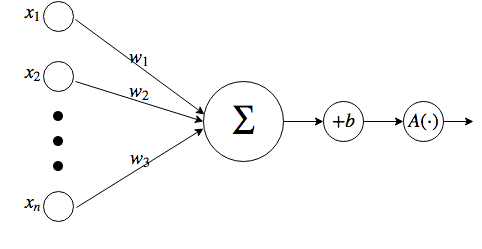
\includegraphics[width=0.6\linewidth]{Perceptron}
   	\end{center}
   	\caption{Схематическое изображение работы одного отдельного нейрона.}
   	\label{tikzpicture: perceptron}
\end{figure}


\indent
\indent
Таким образом, значение на выходе нейрона задается
 выражением \ref{eq:perceptron}.

\begin{equation}\label{eq:perceptron}
    f(\vec{x}) = A(\sum_{i=1}^n x_i w_i + b)
\end{equation}


где $f(\vec{x})$ -- выходное значение нейрона, посчитанное для входов $x_i$,
$w_i$ -- весовые коэффициенты для каждого входа, $b$ -- параметр смещения, 
а $A$ --- нелинейная функция активации. Далее для упрощения повествования
положим $b \equiv 0$.

\subsection{Функции активации}

\indent
\indent
Существуют множество различных функций активации, например, гиперболический
тангенс, логистическая сигмоида или \textit{ReLU}, рисунок \ref{tikzpicture: activations}.

\begin{equation}\label{eq:activations}
	\begin{gathered}
	    A_{1}(x) = th(x) = \frac{e^x - e^{-x}}{e^x + e^{-x}},    \;   th’(x) = {1 - th(x)^2}  \\    
	    A_{2}(x) = \sigma(x) = \frac{1}{1 + e^{-2x}},   \;   \sigma’(x) = \sigma(x)(1 - \sigma(x)) \\
	    A_{3}(x) = ReLU = max(0, x),   \;   ReLU’(x) = \theta(x)
	\end{gathered}
\end{equation}
где $\theta(x)$ -- функция Хэвисайда.

\indent
\indent
Эти функции используются
для добавления нелинейных зависимостей между слоями многослойной модели.
Названные выше функции особенно популярны, 
так как значения их производных либо достаточно просты, либо легко 
выражаются через значения самих функций (выражение \ref{eq:activations}), 
что позволяет быстро вычислять значение производной.

\begin{figure}[h!]
	\begin{center}
		\begin{tikzpicture}
			\begin{axis} [
			    legend pos = north west, 
			    xmin = -2,
			    xmax = 2,
			    minor tick num = 2
			]
			\legend{ 
				$th(x)$, 
				$\sigma(x)$, 
				$ReLU(x)$
			};
			\addplot[blue, line width = 1.5] {tanh(x)};
			\addplot[red, line width = 1.5] {1 / (1 + e^(-2*x))};
			\addplot[green, line width = 1.5] {max(0, x)};
			\end{axis}
		\end{tikzpicture}
	\end{center}
\caption{Функции активации}
\label{tikzpicture: activations}
\end{figure}

\subsection{Полносвязная сеть}

\indent
\indent
Одиночный нейрон не способен выразить сложные в наборе
признаков $\vec{x}$, поэтому нейроны объединяют в слои, а их, в свою 
очередь, в многослойные сети . Рассмотрим сеть,
состоящую из двух слоев нейронов. Пусть количество количество входных признаков
равно $N$, количество нейронов скрытого слоя $P$,
а размер выхода -- $M$, рисунок \ref{tikzpicture: fc_net}. Такая архитектура, 
состоящая из простых линейных слоев, называется полносвязной.
 
\begin{figure}[h!]
    \begin{center}
   	    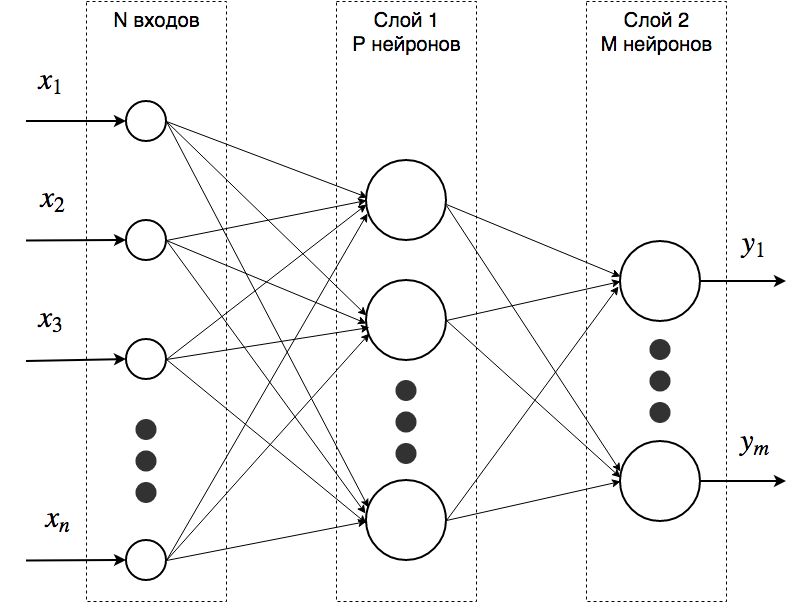
\includegraphics[width=0.9\linewidth]{FC_net}
   	\end{center}
   	\caption{Схематическое изображение полносвязной нейронной сети.}
   	\label{tikzpicture: fc_net}
\end{figure}

Рассмотрев выражение \ref{eq:perceptron} можно увидеть, что 
совокупность значений нейронов на 1 слое может быть получена 
простым матричным умножением входов $\vec{x}$ на матрицу весов
 $W^1$ размера $P \times N$, с последующим поэлементным применением 
функции активации к получившимся значениям. Аналогично, значения нейронов
2 слоя получаются умножением предыдущих значений на весовую матрицу
$W^2$ размером $M \times P$. Таким образом, применение нейросети
ко входу $\vec{x}$ можно задать выражением \ref{eq:forward}.

\begin{equation}\label{eq:forward}
	   \vec{y} = A(W^{2} A(W^{1} \vec{x}))
\end{equation}
где $A(\cdot)$ -- применение нелинейности к каждому элементу входного 
вектора.

\indent
\indent
Если бы мы не добавляли после слоев нелинейность, то выражение \ref{eq:forward}
выродилось бы в простое умножение слева входного вектора $\vec{x}$ на матрицу
$W^{12} \equiv W^{2} W^{1}$. В этом случае модель не смогла бы выучить 
сложные нелинейные зависимости в данных, а добавление дополнительных слоев
не имело бы смысла, т.к. все они могут быть описаны одной матрицей весов.

\indent
\indent
Отметим, что количество весов сети, состоящей из полносвязных слоев, растёт
мультипликативно от их размеров. Поэтому из-за больших вычислительных затрат
 на практике обычно не встречаются по-настоящему глубокие полносвязные архитектуры.
 Один из способов выразить сложные зависимости меньшим количеством слоев ---
 использование сверточных слоёв, о которых будет рассказано позднее.


\subsection{Функции потерь}
\label{section: losses}

\indent
\indent
Близость предсказания сети к правильным ответам оценивается
с помощью функции ошибки, так же называемой 
 функцией потерь \textit{(loss function)}. 
Например, для задачи регрессии в качестве функции потерь
может применяться сумма квадратов отклонений
 (выражение \ref{eq: se}),
 или, в более простом случае -- сумма разностей между выходами модели
  и правильными ответами (выражение \ref{eq:diff});
для задачи классификации обычно используют перекрестную энтропию 
(\textit{cross entropy}, выражение \ref{eq: cross_entropy}).


\begin{equation}\label{eq:diff}
    L_{diff}(\vec{y_{gt}}, \vec{y}) = \sum_{i=1}^M | y^{gt}_{i} - y_{i} |
\end{equation}

\begin{equation}\label{eq: se}
    L_{mse}(\vec{y_{gt}}, \vec{y}) = \frac{1}{2} \sum_{i=1}^M (y^{gt}_{i} - y_{i})^2
\end{equation}
где $\vec{y}$ -- предсказанный моделью $M$-мерный целевой вектор 
признаков, $\vec{y_{gt}}$ -- правильные значения признаков; в общем
случае в задаче регрессии признаки являются вещественными числами
 $\in (- \inf; + \inf )$.

\begin{equation}\label{eq: cross_entropy}
    L_{ce}(y_{gt}, \vec{y}) = - \sum_{i=1}^M \delta_{y_{gt}, i} \log{y_{i}}
\end{equation}
где $i$ -- метка класса (классы пронумерованы натуральными 
числами от $1$ до $M$),
$y_{gt}$ --  правильная метка класса
для рассматриваемого экземпляра данных;
$y_i$ -- предсказанная вероятность того, что 
экземпляру соответствует $i$-й класс;
$\delta_i$ -- символ Кронекера. 


\indent
\indent
Исходя из постановки решаемой задачи, можно составить и другие функции ошибок, но
они обязательно должны быть дифференцируемыми.
Это необходимо условие, чтобы использовать метод обратного распространения
ошибки для обучения модели.


\subsection{Обучение нейронных сетей}
% https://habr.com/ru/company/ods/blog/344116/
% https://ru.wikipedia.org/wiki/Метод_обратного_распространения_ошибки

\indent
\indent
Обучение нейронной сети -- это процесс изменения весовых
коэффициентов между нейронами, направленный на уменьшение
 значения функции потерь на тренировочном наборе данных $\{ \vec{x} | \vec{y} \}$. 
 Мы рассмотрим базовую реализацию такого процесса -- алгоритм 
 стохастического градиентного спуска. Мы будем подавать на вход модели
 размеченные тренировочные данные, объединенные в  небольшие партии 
 \textit{(batches)}. Идея состоит в том в том, чтобы после каждой такой партии
добавлять ко всем весам поправку, противоположную градиенту от функции потерь
(выражение \ref{eq: grad_idea}). 
Отметим, что метод называется стохастическим, так как веса 
модели обновляются после каждой партии данных. Из-за этого
направление, в котором делается шаг по профилю функции потерь,
не является оптимальным для обучающего набора данных в целом.
Можно интерпретировать этот факт как добавление шума
к вычисляемому градиенту, отсюда и стохастичность в названии.


\begin{equation}\label{eq: grad_idea}
    w_{i, j} \leftarrow w_{i, j} - \Delta w_{i,j} = - v \frac{\partial L}{\partial w_{i, j}}
\end{equation}
где $v \in (0; 1)$ -- параметр, отвечающий за скорость обучения \textit{(learning rate)}.

Для начала положим, что $j$ является 
нейроном последнего слоя. Обозначим $S_{j} = \sum_{i} w_{i, j} x_{i}$ и
распишем производную из выражения \ref{eq: grad_idea}.

\begin{equation}\label{eq: derivs}
    \frac{\partial L}{\partial w_{i, j}} = 
    \frac{\partial L}{\partial S_j} \frac{\partial S_j}{\partial w_{i, j}} =
    x_i \frac{\partial L}{\partial S_j} =
    x_i \frac{\partial L}{\partial y_j} \frac{\partial y_j}{\partial S_j} =
    x_i \frac{\partial L}{\partial y_j}  \frac{\partial A(S)}{\partial S} | S_j
\end{equation}

Чтобы сосчитать производные в выражении \ref{eq: derivs} осталось выбрать какие-то конкретные
функции потерь и активации. Выберем в качестве функции активации $A$ 
логистическую сигмоиду $\sigma$ (формула \ref{eq:activations}), а в качестве функции потерь
$L$ -- квадратичное отклонение (формула \ref{eq: se}). После подстановки получим
окончательную формулу для обновления весов последнего слоя (формула \ref{eq: weights_upd}).

\begin{equation}\label{eq: weights_upd}
    w_{i, j} \leftarrow w_{i, j} - 2 v x_i y_j (1 - y_j) (y^{gt}_j - y_j)
\end{equation}

Рассмотрим случай, когда $j$-й узел находится во внутренних слоях и 
у него есть выходы (обозначим их как \textit{childrens(j)}).

\begin{equation}\label{eq: childrens}
    \frac{\partial L}{\partial S_j} = 
    \sum_{k \in childrens(j)} \frac{\partial L}{\partial S_k} \frac{\partial S_k}{\partial S_j} 
\end{equation}


\indent
\indent
В выражении \ref{eq: childrens} можно явно сосчитать 
$\frac{\partial S_k}{\partial S_j}$, в нашем случае мы получим 
$2 w_{j, k} y_j (1 - y_j)$, а $\frac{\partial L}{\partial S_k}$ -- это поправка для весов, вычисленная для узла 
следующего уровня (с точностью до коэффициента $-v x_i$). Таким образом, мы можем вычислить
поправку для весов нейронов последнего уровня (выражение \ref{eq: weights_upd}), и использовать
её, чтобы вычислить поправки для остальных уровней
(выражение \ref{eq: childrens}). Из-за вычислений такого вида
 данный подход так же называют алгоритмом обратного распространения ошибки \textit{(backpropogation)}.
 

\subsection{Сверточные нейронные сети}
% https://habr.com/ru/company/ods/blog/344008/

\indent
\indent
Сверточные нейронные сети \textit{(Convolution neural network, CNN)} --- 
это искусственные нейронные сети специального вида,
изначально сконструированные для 
обработки изображений, хотя в настоящее время спектр их применения 
значительно расширился. Как следует из названия, основной таких сетей 
являются сверточные слои \textit{(convolutional layers)}.

\indent
\indent
 Для начала на простом примере рассмотрим,
 как устроен результат $G$ применения свертки c ядром $h$ 
 к матрице  $F$, формула \ref{eq: conv}. 

\begin{equation}\label{eq: conv}
    \begin{gathered}
        G = F \otimes h \\
	    G_{i, j} = \sum_{a=-n}^{n} \sum_{b=-n}^{n} h_{a, b} F_{s*i - n, s*j - n} \qquad
	    \forall i \in (1..I), \forall j \in (1..J) \\
    \end{gathered}
\end{equation}
где $F$ --- матрица размером $I \times J$;
$h$ --- ядро свертки размером $2n+1 \times 2n+1$;
$s$ --- шаг, с которым свертка "передвигается" по матрице $F$ \textit{(stride)};
$G$ --- матрица размером $I \times J$, результат свертки.

\indent
\indent
Обычно ядро свертки $h$ --- это небольшая матрица весов размером
 $3\times3, 5\times5$ или $7\times7$. В качестве матрицы $F$ может выступать
 некоторое изображение (в приведенном примере --- в оттенках серого),
  или карта признаков \textit{(feature map)}, полученная 
путём сворачивания изображения с ядрами других сверток.
Графическая иллюстрация
к операции свертки приводится на рис. \ref{tikzpicture: conv}.


\begin{figure}[h!]
    \begin{center}
   	    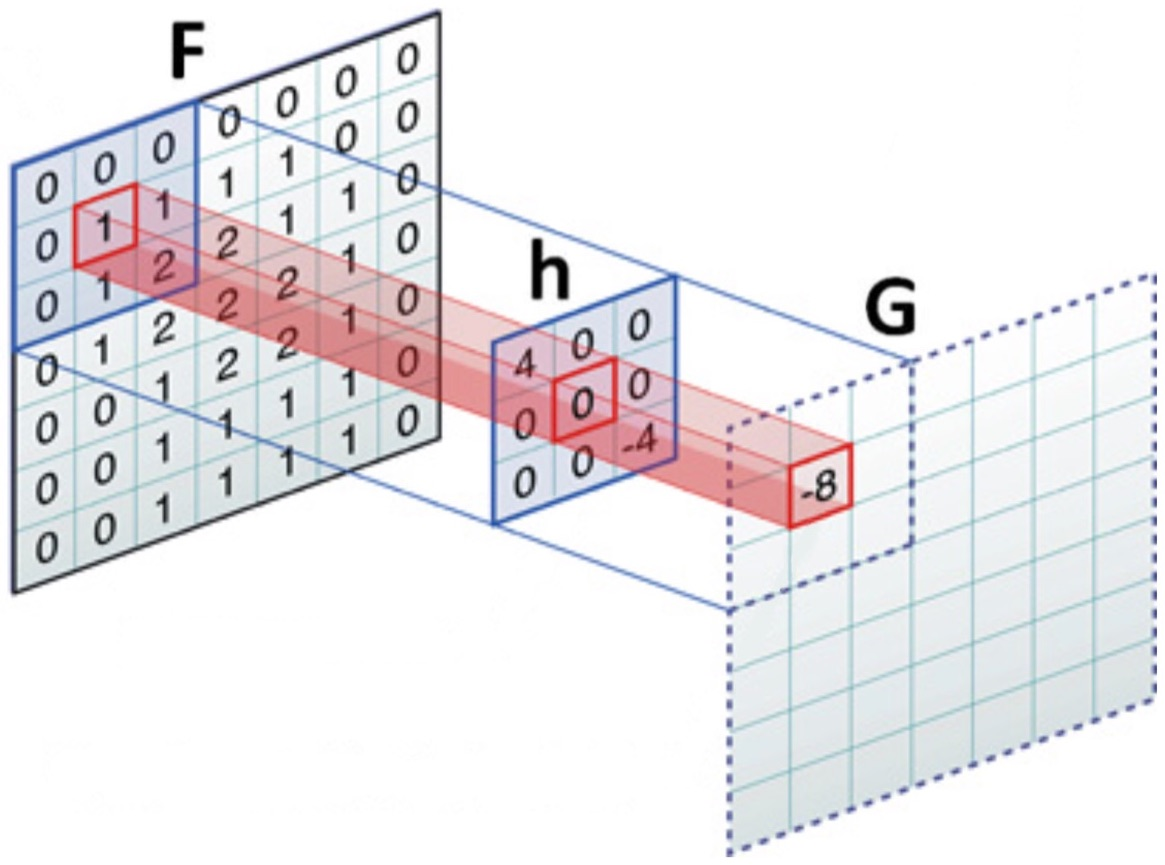
\includegraphics[width=0.6\linewidth]{conv}
   	\end{center}
   	\caption{Свертка матрицы $F$ с ядром свертки $h$.}
   	\label{tikzpicture: conv}
\end{figure}


\indent
\indent
В классическом компьютерном зрении известны конкретные числовые
значения элементов матрицы $h$ для ряда сверток 
специального вида. Например, ядро (чаще называемое оператором) Собеля 
позволяет выделять границы на изображениях, а ядро (чаще
называемое фильтром) Гаусса используется для устранения шума
и размытия контуров на изображении. Идея добавления сверточных слоев в 
 нейронные сети строится на том, что сеть сама в процессе
обучения методом обратного распространения ошибки "выучит" подходящие
для решения конкретной задачи весовые коэффициенты в обучаемых ядрах.

\indent
\indent
Кроме того, обычно вместе со сверточными слоями используются такие 
слои как \textit{Pooling}, \textit{Softmax}, 
\textit{BatchNormalization}\cite{batchnorm}  и \textit{Dropout}\cite{dropout}.


\subsection{Используемые сверточные архитектуры}
\label{section:archs}

\indent
\indent
В данной работе используются следующие архитектуры нейронных сетей:


\begin{itemize}

    \item Residual netwrotk (ResNet) ---
    одна из самых популярных в настоящее время архитектур,
    предложенная в статье от \textit{Microsoft} \cite{resnet}.
    Основная идея состоит в добавлении конкатенации выходов
    слоя с номером  $i$ и слоя $i - 2$ (такая процедура
    получила название \textit{skip connection}. Таким образом авторы
    успешно решают проблему 
    обучения глубоких сетей --- затухание градиентов.
    
    \item {Inception} --- топология, предложенная исследователями 
    из компании \textit{Google} \cite{inception}. Основную идею
    можно выразить фразой "сеть внутри сети". Авторы 
    конструируют сеть из блоков \textit{(inception modules)} и
    используют свертки $(1 \times 1)$.
    
    \item {VGG} --- относительно глубокая сеть, авторы которой предложили
    решение проблемы обучения огромного количества параметров
    сверточных слоев \cite{vgg}. Вместо сверток с ядрами $(7 \times 7)$ и
    $(9 \times 9)$ они используют несколько сверток $(3 \times 3)$, уменьшив
    количество весов, при этом сохранив 
    площадь восприятия \textit{(reception field)}.
    
\end{itemize}

\indent
\indent
Для перечисленных выше архитектур в открытом доступе находятся 
веса обученных моделей, тренированных на классификации 1000
категорий датасета \textit{ImageNet}\cite{imagenet}. В настоящей работе
эти веса используются для инициализации слоев обучаемых моделей
(для этого требуется заменить размер выходного слоя на количество
категорий, рассматриваемых в решаемой задаче).
Такой подход имеет широкое распространение 
и называется \textit{fine-tuning}, он позволяет значительно ускорить
тренировочный процесс и, иногда, увеличить конечную точность модели.




\newpage
\section{Работа с данными}


\subsection{База семантических связей WordNet}

\indent
\indent
Обсуждение работы с данными наиболее логично начать с описания базы знаний
\textit{WordNet'а}, который использовался и авторами датасета \textit{SUN},
и автором настоящей работы. Составители датасета \textit{SUN} использовали
\textit{WordNet} для создания иерархии названий сцен (локаций). А в настоящей работе
он используется для объединения названий локаций в обобщающий домен
и для поиска синонимов к предлагаемым пользователю тегам.

\indent
\textit{WordNet} --- это электронный словарь/семантическая сеть для английского
языка. Он содержит 4 подсети: для глаголов, существительных, прилагательных и
наречий. Узлами сети являются не отдельные слова, а синсеты \textit{(synset)},
объединяющие слова со схожим значением. Таким образом, слова, имеющие 
несколько значений могут быть включены в несколько синсетов.

Синсеты связаны между собой различиными отношениями. 
Например, один синсет может выступать по отношению к другому в роли гиперонима, гипонима, меронима, антонима и т.д. todo 

Кроме того, между синсетами можно вычислять различные меры близости.

\begin{itemize}

    \item \textit{Path similarity} --- показывает, насколько близки пути до 
    синсетов в общем графе \textit{WordNet'а}.
    
    \item 
    
    
\end{itemize}


\subsection{Датасет SUN}

\indent
\indent
Набор данных \textit{SUN (Scenes Understunding Dataset)} впервые был 
представлен исследовательскому сообществу в 2010 году на 
конференции CVPR, посвященной компьютерному зрению. Одновременно
авторы опубликовали статью \cite{sundata}, в которой приводят различные
статистики по датасету; описывают процесс сбора и разметки данных; 
применяют к задаче распознавания сцен лучшией из имеющихся
на тот момент методов. 

\indent
Датасет представляет собой набор фотографий, на каждой из которых запечатлена
одна из 908 локаций, примеры приведены на рисунке \cite{tikzpicture: sun}. Причем
часть локаций представлена в двух
вида: снаружи и изнутри. Чтобы отличить эти два случая к названиям сцен добавляются слова \textit{outdoor} или \textit{exterier} и \textit{indoor} или \textit{interier} соответственно.
Кроме того, в 2012 году авторы для части изображений представили разметку 
на уровне объектов: были предоставлены маски для 300 тыс. объектов, относящихся
к одной из 5 тыс. категорий.

\indent
Наконец, авторы оставили только хорошо интепретирующиеся классы сцен, 
содержащие хотя бы 100 примеров, после чего организовали на этом
наборе данных соревнование по машинному обучению. Итоговый датасет
для решения задачи классификации,
который и будет использоваться в данной работе,
содержит 108754 изображений (около 40 ГБ на жестком диске), каждое 
из которых отнесено к одному из 397 классов.

\begin{figure}[h]
    \begin{center}
   	    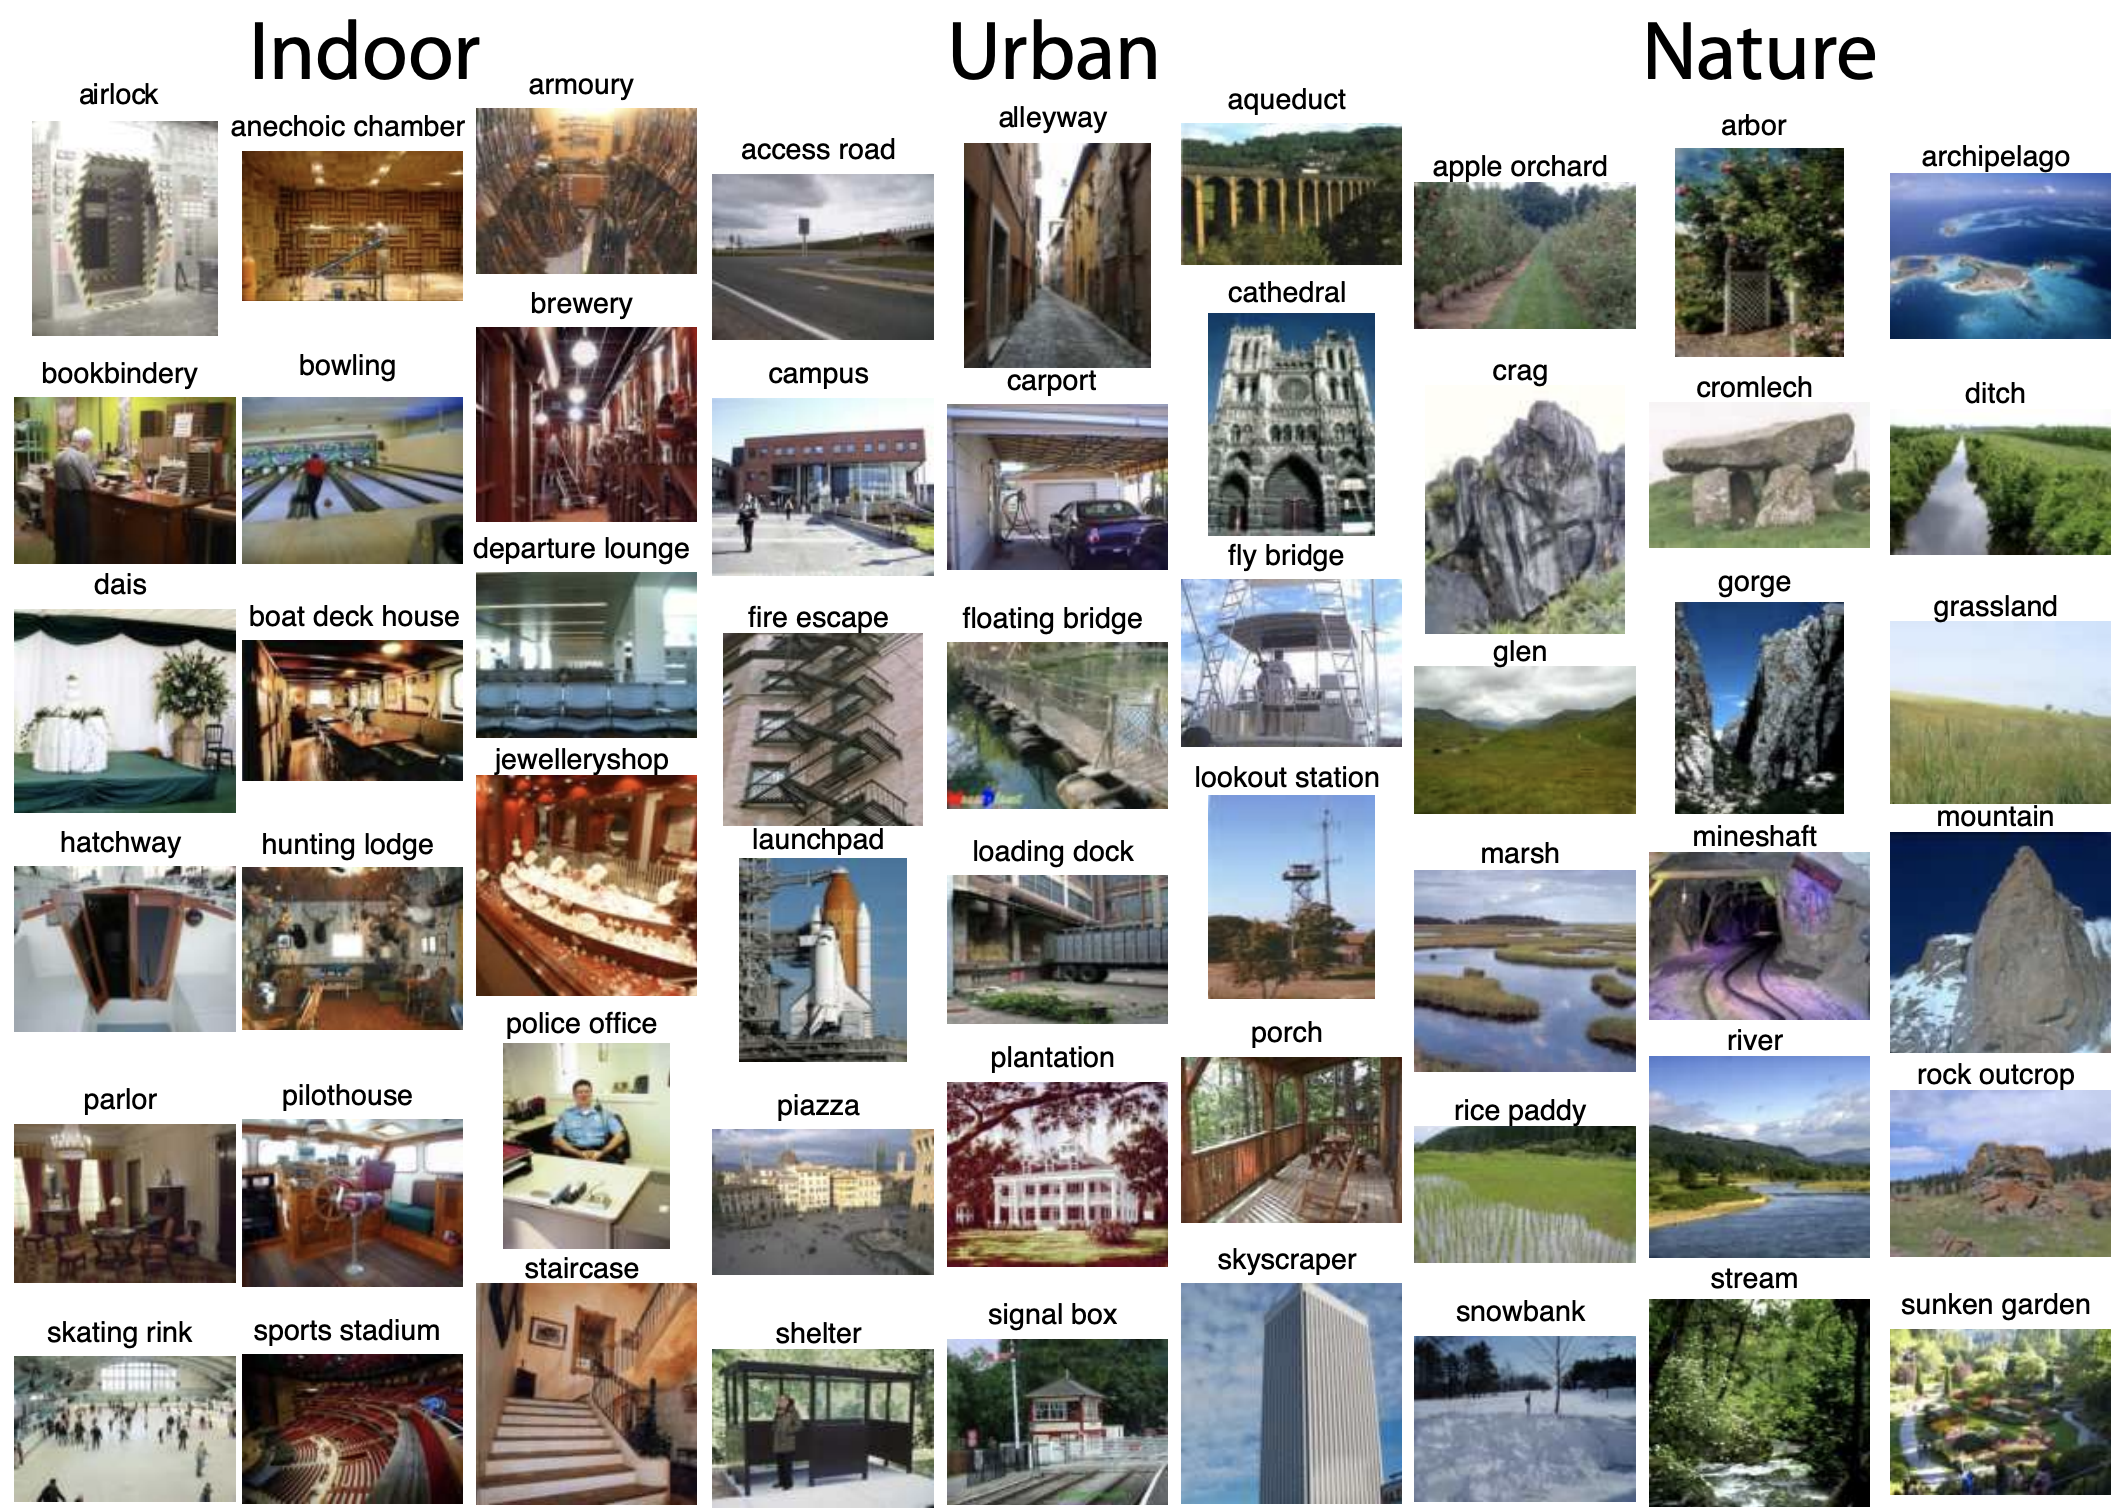
\includegraphics[width=0.95\linewidth]{Sun}
   	\end{center}
   	\caption{Примеры размеченных фотографий из датасета \textit{SUN}.}
   	\label{tikzpicture: sun}
\end{figure}

Ознакомиться с другими изображениями из датасета \textit{SUN} можно через 
интерактивный веб-обозреватель\footnote{groups.csail.mit.edu/vision/SUN/}, которым
можно воспользоваться для просмотра упорядоченных изображений как 
по сценам, так и по объектам.


\subsection{Адоптация датасета SUN}

\indent
\indent
Как было сказано во введении, названия локаций (сцен) из датасета \textit{SUN} не 
являются сами по себе популярными тегами из социальных сетей. Поэтому 
прежде всего необходимо выполнить сопоставление. Условно можно
разбить процедуру сопоставления на 2 части: объединение исходных классов 
датасета \textit{SUN} в семантические домены и сопоставление полученных доменов
с популярными хэштегами. В качестве источника хэштегов была выбрана социальная
сеть \textit{Instagram}\footnote{www.instagram.com}, ориентированная на обмен фото
и видео контентом между пользователями.

\indent
Итак, предварительно необходимо очистить названия классов \textit{SUN} от служебных
слов и символов, таких как \textit{indoor, outdoor, exterier, interier}, знаков "/" и 
однобуквенных алфавитных указателей. Затем для полученных слов или 
словосочетаний подбирается соответсвующий синсет из базы знаний \textit{Wordnet}.
Далее для синсетов находились гиперонимы, которые либо уже были достаточно
абстрактны, чтобы представлять собой часто встречающийся тег, либо 
автор работы находил для синсетов обобщающее понятие вручную.
Несколько примеров приведено в таблице~\ref{tabular: mapping}.


% Таблица о сопоставлении классов и тегов
\begin{table}[h]
    \begin{center}
        \begin{tabular}{c | c| c | c | c}
            \hline
            № & Исходное название & Синсет & Гипероним & Хэштег \\
            \hline
    
            1 & /s/shoe\_shop & shoe shop & shop & \htag{shopping} \\
    
            2 & /t/toyshop & toyshop & shop & \htag{shopping} \\
   
            3 & /v/volleyball\_court/indoor & volleyball court & court & \htag{sport} \\
    
            4 & /w/wrestling\_ring/indoor & wrestling ring & ring  & \htag{sport} \\
    
            5 & /r/rainforest & rain forest & forest & \htag{forest} \\
            
            6 & /p/pantry & pantry & storeroom & ? \\
   
            \hline
        \end{tabular}
    \end{center}
    \caption{Сопоставление искомых классов и хэштегов.}
    \label{tabular: mapping}
\end{table}


\indent
Из таблицы~\ref{tabular: mapping} видно, что некоторые синсеты имеют общие
гиперонимы. Кроме того, некоторые гиперонимы без каких-либо
дополнительных изменений могли быть использованы пользователями в качестве 
тегов. Таким образом, использование гиперонимов позволило немного уменьшить
количество ручной работы. Так же в таблице~\ref{tabular: mapping} приведен пример,
когда для локации сложно подобрать какой-то подходящий и широко распространенный
тег.  В итоге использовалось около половины из  \textit{397}
искомых классов датасета \textit{SUN}, каждому из которых удалось поставить
в соответсвие один из \textit{20} популярных хэштегов. В данной работе 
популярными считаются теги, использованные в сети
\textit{Instagram} более \textit{10 млн.} раз. При этом среднее число упоминаний 
отобранных тегов составило \textit{100 млн.} раз, а
максимальное --- \textit{450 млн.}. Полная информация о частоте встречаемости
для всех хэштегов приведена на рисунке ~\ref{tikzpicture: tags_counts}.


% Гистограмма встречаемости хэштегов
\begin{center}
    \begin{figure}[h]
    \begin{tikzpicture}
    \label{tags_counts}
        \begin{axis}[
            ylabel = Число использований млн.,
            x tick label style={rotate=90,anchor=east},
            width = 0.7\paperwidth,
            height = 0.4\paperheight,
            symbolic x coords=
            {
                art,
                nature,
                beach,
                sky,
                home,
                shopping,
                artchitecture,
                water,
                sport,
                street,
                car,
                cafe,
                garden,
                urban,
                forest,
                bar,
                church,
                building,
                road,
                airport,
                entertainment,
                science
            },
            xtick=data
          ]
            \addplot[ybar,fill=blue] coordinates {
                (art, 450)
                (nature, 390)
                (beach, 210)
                (sky, 190)
                (home, 115)
                (shopping, 100)
                (artchitecture, 97)
                (water, 65)
                (sport, 60)
                (street, 55)
                (car, 55)
                (cafe, 45)
                (garden, 41)
                (urban, 32)
                (forest, 30)
                (bar, 25)
                (church, 25)
                (building, 23)
                (road, 17)
                (airport, 14)
                (entertainment, 10)
                (science, 10)
            };
        \end{axis}
    \end{tikzpicture}
    \caption{Встречаемость предсказываемых хэштегов в социальной сети \textit{Instagram}.}
    \label{tikzpicture: tags_counts}
    \end{figure}
\end{center}


\indent 
Отметим, что автор предпринял несколько попыток произвести процедуру 
адаптации разметки датасета \textit{SUN} полностью автоматически, 
но они оказались неудачными. 


\indent
\indent
Первая попытка --- обобщить искомые классы, используя метод \textit{topic\_domains},
который доступен для синсетов в \textit{python} реализации API к 
базе \textit{WordNet}. Например, для синсета
\textit{basketball\_court.n.01}, который определяется как 
\textit{the court on which basketball is played}, 
вызов данного метода возвращает \textit{basketball.n.02}, который определяется так:
\textit{a game played on a court by two opposing teams of 5 players;
points are scored by throwing the ball through an elevated horizontal hoop}.
К сожалению, проблема заключалась в том, что для подавляющего числа названий 
локаций \textit{topic\_domains} возвращал пустое значение, т.е. для этих синсетов
авторами базы знаний не было назначено доменов.


\indent
\indent
Вторая попытка аналогичная первой, но использовалась сторонняя база знаний
\textit{WordNet Domains}\footnote{http://wndomains.fbk.eu/}. К сожалению, такое
расширение базы доменов не позволило решить проблему, описанную выше.


\indent
\indent
Третья идея заключась в использовании информации о семантической близости 
синсетов, в частности, API \textit{WordNet'a} позволяет для любых двух синсетов
вычислить степень похожести несколькими способами:
\textit{jcn\_similarity, lch\_similarity, res\_similarity, wup\_similarity}.
Для разных видов измерения расстояния были вычислены матрицы попарных дистанций,
на основе которых производилась иерархическая кластеризация с различными
гиперпараметрами
 (например, класторизация по заданному максимальному расстоянию в кластере, 
по заданному количеству кластеров). К сожалению, автору не удалось получить кластеры,
большую часть которых можно было бы без труда "озаглавить" 
каким-либо популярным хэштегом.


\indent
\indent
Таким образом, процедуру сопоставления всех 
\textit{397} искомых классов датасета \textit{SUN} и хэштегов из социальной сети \textit{Instagram}
пришлось произвести в полуручном режиме (опираясь только на гиперонимы),
как это было описано выше в данном разделе.


\indent
\indent
Приведем пример такого сопостовления. В таблице \ref{tabular: sport_classes} 
перечислены названия локаций, которым поставлен в соответсвие хэштег \htag{sport}:

\begin{table}[ht!]
    \begin{center}
        \begin{tabular}{c | c | c}
            /w/wrestling\_ring/indoor &
            /a/athletic\_field/outdoor &
            /b/badminton\_court/indoor
            \\
            /b/ball\_pit &
            /b/baseball\_field &
            /b/basketball\_court/outdoor
            \\
            /b/boxing\_ring &
            /b/bullring &
            /g/golf\_course
            \\
            /g/gymnasium/indoor &
            /m/martial\_arts\_gym &
            /r/racecourse
            \\
            /r/riding\_arena &
            /s/ski\_lodge &
            /s/ski\_resort
            \\
            /s/ski\_slope &
            /s/squash\_court &
            /s/stadium/baseball
            \\
            /s/stadium/football &
            /s/swimming\_pool/indoor &
            /s/swimming\_pool/outdoor
            \\
            /t/tennis\_court/indoor &
            /t/tennis\_court/outdoor &
            /v/volleyball\_court/indoor
            \\
            /v/volleyball\_court/outdoor          
        \end{tabular}
    \end{center}
    \caption{Список классов датасета \textit{SUN}, которым сопоставлен хэштег \htag{sport}.}
    \label{tabular: sport_classes}
\end{table}

Файлы с полной информацией об итоговом сопоставлении можно найти в 
репозитории автора\footnote{github.com/AlekseySh/scenes}.


\newpage
\section{Численные эксперименты}

\indent
\indent
В данной главе мы обсудим экспериментальную часть работы, начиная от
архитектуры программы и заканчивая обсуждением полученных результатов.



\subsection{Архитектура программы}

\indent
\indent
Основная часть программы, выполняющая обучение и тестирование модели
 состоит из стандартного для фреймворка \textit{pytorch} набора 
 взаимосвязанных компонент (классов). Перечислим их:


\begin{itemize}

	\item
	\textit{Module} --- описывает непосредственно вычислительный граф нейросети. 
	Здесь указаны параметры и количество всех слоев, описаны связи между ними.
	
	\item
	\textit{Dataset} --- позволяет итерироваться по набору данных и объединять их в 
	батчи для подачи на вход нейросети.
	
	\item
	\textit{Loss} --- вычисляет функцию ошибки/потери между предсказанными 
	моделью  и правильными значениями целевой переменной.
	
	\item
	\textit{Optimizer} --- совершает шаг градиентого спуска на заданное расстояние,
	которое определяется скоростью обучения \textit{(learning rate)}. А именно,
	изменяет веса модели так, чтобы уменьшить среднюю ошибку для очередного
	переданного на вход модели батча данных.
	
	\item
	\textit{Scheduler} --- изменяет скорость обучения модели \textit{(learning rate)}
	с течением времени по заданному правилу.
	
	\item
	\textit{Stopper} --- останавливает тренировку при выполнении заданного 
	условия, например, если в течение последних \textit{n} эпох не произошло
	увеличения точности модели хотя бы на $\epsilon$.
	
	\item
	\textit{MetricsCalculator} --- оценивает точность модели на некоторой размеченной
	подвыборке данных по заданным метрикам.
	
	\item
	\textit{TensorboardX}  --- система для визуального логирования обучения
	модели; позволяет строить графики изменения функции ошибки, метрик и
	выводить любые другие пользовательские изображения.
	
	\item
	\textit{Trainer} -- объединяет воедино компоненты, названные выше. Обучает
	модель эпоху за эпохой, с заданной частотой проверяет текущую точность
	на тестовом подмножестве данных. Останавливает тренировку по
	достижению некоторого критерия. Сохраняет промежуточные
	веса модели. Визуализирует процесс обучения.
 
 \end{itemize}


 \indent
 \indent
 Взаимосвязь между компонентами программы можно проследить на 
  рисунке \ref{tikzpicture: programm}.

\begin{figure}[h!]
    \begin{center}
   	    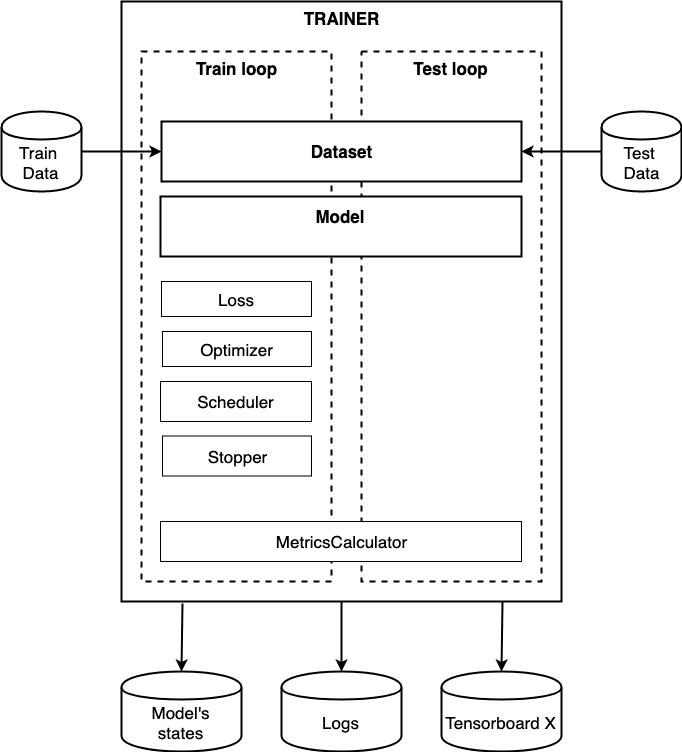
\includegraphics[width=0.95\linewidth]{Programm}
   	\end{center}
   	\caption{Структура программы для тренировки и обучения модели.}
   	\label{tikzpicture: programm}
\end{figure}


\subsection{Выбор метрики}

\indent
\indent
Прежде всего необходимо определиться, как количественно будет оцениваться
точность модели.Мы случайно выбрали 80\% данных 
для тренировки моделей, и 
20\% для их тестирования. В качестве метрик будем использовать 
классические для задачи классификации точность
 (\textit{accuracy}, не путать с \textit{precision}) и взвешенную точность:
выражения \ref{eq:accuracy} и \ref{eq:w_accuracy}.


\begin{equation}\label{eq:accuracy}
	   acc(\vec{y^{gt}}, \vec{y}) = \frac{1}{N}\sum_{i=1}^{N} \delta_{y_i^{gt}, y_i}
\end{equation}
где $\vec{y^{gt}}$ --- вектор номеров классов длинной $N$, 
$\vec{y}$ --- вектор предсказанных номеров классов длинной $N$,
$N$ --- количество рассматриваемых примеров,
$\delta$ --- символ Кронекера.

\begin{equation}\label{eq:w_accuracy}
	   acc_w(\vec{y^{gt}}, \vec{y}) = 
	   \frac{1}{C} \sum_{c}
	   \frac{1}{N_c}\sum_{\{i: y_i^{gt}\equiv c\}} \delta_{y_i^{gt}, y_i}
\end{equation}
где $N_c$ --- количество примеров из класса $c$, $C$ --- количество классов.
 

\indent
\indent
Таким образом, чтобы посчитать точность достаточно просто разделить
количество правильных ответов на общее количество ответов. Чтобы посчитать
взвешенную точность, необходимо вычислить точность для каждого класса
в отдельности, а затем усреднить полученные значения. В случае, если распределение
по классам в значительной степени неравномерное, отсутствие такого усреднения
приведет к тому, что значение метрики будет определяться точностью модели на
нескольких наиболее представленных классах. В данной работе мы будем
смотреть на значения обеих вариантов точности, но для принятия
решений о выборе модели приоритетной является взвешенная точность, так как в нашем наборе данных присутствует большой по размеру класс \textit{other}.


\section{Ход экспериментов}

\indent
\indent
Чтобы обучить модель оптимальным образом, сначала проведем серию
легковесных (с вычислительной точки зрения) экспериментов, чтобы определиться 
со значениями основных гиперпараметров. Затем попробуем улучшить целевую метрику
для лучшей модели, полученной на первом шаге.

\indent
\indent
Начнём с топологии нейронной сети. Будем выбирать из трех семейств архитектур:
 \textit{ResNet}, \textit{Inception} и \textit{VGG}; подробнее см. в разделе \ref{section:archs}.
Чтобы ускорить эксперименты уменьшим размер всех изображений до
$256 \times 256$ пикселей и не будем использовать аугментации во время тренировки.
Прекратим обучение после 50-ти
эпох\footnote{\textit{Эпохой} в машинном обучении называется один полный проход по
обучающему набору данных в процессе тренировки.}, либо остановимся досрочно,
если в течение 5-ти последних эпох от текущей не будет улучшено 
значение метрики хотя бы на 0.5\%. В качестве функции потерь используем
 перекрестную энтропию (см. раздел \ref{section: losses}),
 а в качестве оптимизатора параметров 
нейронной сети --- \textit{Adam} \cite{adam}, т.к. он не требует тонкой настройки
параметров. Кроме того, отследим время, которое 
понадобилось на обучение модели до остановки эксперимента 
по названному выше критерию. В качестве финального состояния модели выберем
то, которое соответствует моменту достижения максимального значения метрики
на тестовой выборке (это совсем не обязательно происходит на последней эпохе).


\begin{table}[h!]
    \begin{center}
        \begin{tabular}{c | c| c | c | c}
            \hline
            № & Архитектура & Точность & Взвешенная точность  & Время [мин] \\
            \hline
    
            1 & Inception v3 & 0.743 & 0.667 & 239 \\
            
            2 & VGG 11 & 0.678 & 0.565 & 154 \\
            
            3 & VGG 13 & 0.637 & 0.478 & 450 \\
            
            4 & ResNet 18 & 0.692 & 0.602 & 35 \\
            
            5 & ResNet 34 & 0.703 & 0.634 & 119 \\
            
            6 & ResNet 50 & 0.659 & 0.593 & 114 \\
    
            \hline
        \end{tabular}
    \end{center}
    \caption{Сравнение метрик для различных архитектур.}
    \label{tabular: arch_compare}
\end{table}


\indent
\indent
Как видно из результатов предварительных экспериментов
(таблица \ref{tabular: arch_compare}), наибольшую
точность показала архитектура \textit{Inception v3}. При этом 
\textit{ResNet34} уступает в точности незначительно, но требует
в 2 раза меньше времени на обучение, поэтому мы остановим свой
выбор на этой модели. 


Теперь попытаемся улучшить точность базовой модели,
используя различные техники тренировки и изменяя основные гиперпараметры.

\indent
\textbf{Оптимизатор}

\indent
Используем другой оптимизатор, например, \textit{SGD} с 
разными значениями скоростей обучения (\textit{learning rate}).
Кроме того, попробуем изменять скорость обучения в процессе тренировки:
будем её постепенно понижать и повышать.
Подразумевается, что такой подход может
помочь вывести функцию потерь из локального минимума. Данный
метод описан в статье 2017 года
\textit{Stochastic gradient descent with Warm Restarts}~\cite{cosine},
хотя его основная идея возникла ещё в 1983 году в публикации
\textit{Optimization by simulated annealing}~\cite{annealing}. В соответствии со
статьёй, скорость обучения изменяется по формуле \ref{eq:cosine}.

\begin{equation}\label{eq:cosine}
    lr_i = lr_{min} + \frac{1}{2} (lr_{max} - lr_{min}) (1 + \cos(\frac{i}{T} \pi ))
\end{equation}
где $lr$ -- скорость обучения,
$lr_{min}$ -- минимальная скорость обучения,
$lr_{max}$ -- максимальная скорость обучения,
$i$ -- номер текущей эпохи,
$T$ -- полупериод изменения скорости обучения. 

\indent
В настоящей работе использованы два набора параметров:
$lr_{min} = 0.001$, $lr_{max} = 0.1$ и $T = 3$ и
$lr_{min} = 0.001$, $lr_{max} = 0.1$ и $T = 50$. 
В первом случае мы получаем так называемый косинусный отжиг,
так как скорость обучения то увеличивается, то уменьшается.
Второй набор параметров соответствует плавному
уменьшению скорости обучения в течение всей тренировки:
это может помочь быстро найти примерный регион,
где находится глобальный
минимум целевой функции, а затем уточнить его местоположение.
Соответствующие графики изменения
скорости обучения приведены на рисунке \ref{tikzpicture: cosine}.
Разумеется, понять,
какая из эвристик окажется лучшей в конкретном случае, поможет
только эксперимент.


\begin{figure}[h]
    \begin{center}
   	    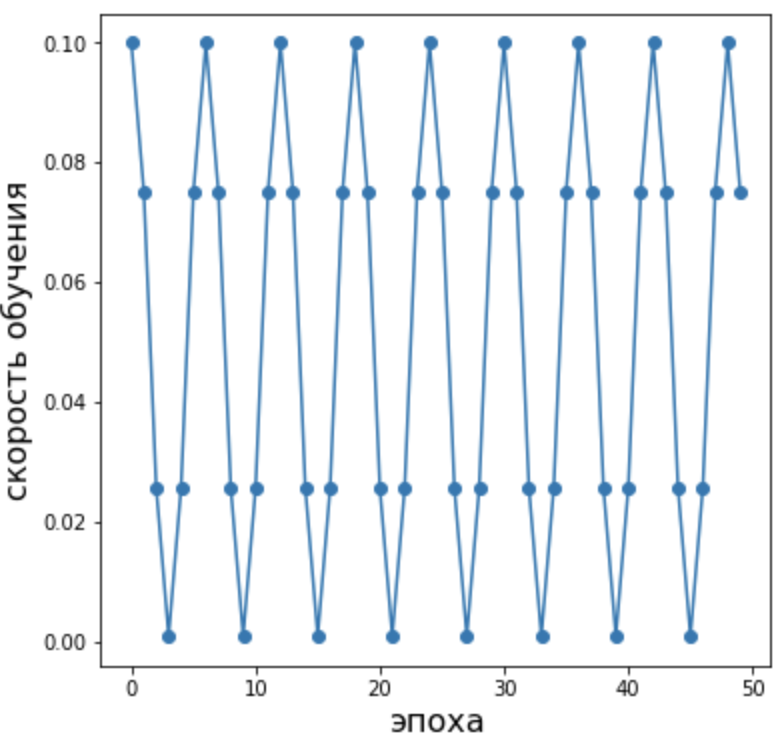
\includegraphics[width=0.5\linewidth]{cosine}
   	\end{center}
   	\caption{Изменение скорости обучения в процессе тренировки.}
   	\label{tikzpicture: cosine}
\end{figure}


\indent
\textbf{Размер изображений}

\indent
Попробуем уменьшать изображения не так сильно, 
до разрешения $512 \times 512$ вместо $256 \times 256 $.
С одной стороны, это сохранит больше информации, но с другой, увеличит 
количество пикселей в 4 раза, что уменьшит размер
батча\footnote{\textit{Батчом} называется набор примеров, который передаётся
модели на обработку за один раз. При работе с изображениями размер батча 
ограничивается размером памяти видеокарты, на которой происходят вычисления.
Как правило, очередной шаг оптимизатора совершается после
прохождения батча, а не отдельного примера.}
и замедлит тренировку.
Поэтому необходимо соблюсти баланс между приростом точности,
которого можно добиться использованием изображений большего размера,
и увеличением времени тренировки.

    
\indent
\textbf{Тренировочные аугментации}

\indent
Применим технику \textit{train time augmentations}, заключающуюся
в намеренном случайном искажении изображений, поступающих на вход модели 
в процессе обучения. Такие преобразования позволяют искусственно
раздуть размер тренировочного набора данных, увеличить его 
вариативность, что, в свою очередь, помогает бороться с переобучением
%footnote
модели\footnote{Переобучением называется ситуация, когда модель
запомнила правильные ответы для примеров из тренировочной выборки,
но не приобрела обобщающую способность. Другими словами, это ситуация,
когда модель имеет хорошее значение метрики на тренировочном наборе,
но очень плохое на тестовом.}.
%footnote
Но возникает вопрос о силе применяемых искажений.
Если трансформации слишком слабы, модель быстро адаптируется
 и её обобщающая 
способность не будет улучшена. Если слишком сильны, то визуальные паттерны, по
которым можно было бы классифицировать изображение, исчезнут. 
Кроме того, чтобы было удобно подбирать подходящую степень искажений,
необходимо каким-то образом количественно её охарактеризовать.
Поступим следующим образом:
для каждого применяемого преобразования выберем некоторое базовое значение 
параметра, соответствующее преобразованию средней силы. 
Затем, одновременно для всех преобразований, будем изменять значения параметров,
в $k$ раз увеличивая или уменьшая выбранные базовые значения.
Таким образом, при $k = 1$ используются трансформации 
с базовыми значениями параметров, при $k = 2$ с удвоенными 
значениями параметров и так далее. Кроме того, вероятность применить то или
иное преобразование так же задаётся параметрически:
$p = 0.4 + 0.1k$.
Перечислим используемые трансформации
и формулы для вычисления их параметров:

\begin{itemize}

    \item Поворот на угол от $-10k$ до $+10k$ градусов.

    \item Из изображения вырезается прямоугольник, линейный размер
    которого выбирается от $1 - 0.1k$ до $1$ размера изображения.
    
    \item Перенос на величину от $0$ до $0.1k$ от линейного
    размера изображения (по вертикали и горизонтали).
    
    \item Сдвиг на величину от $0$ до $0.05k$ от линейного
    размера изображения
    (по вертикали и горизонтали).
    
    \item Изменение отношения сторон в $s$ раз, где $s$ меняется
    от $1 - 0.1k$ до $1 + 0.1k$ от размера изображения.
    Причем большей стороной может оказаться как высота,
    так и ширина изображения.
    
    \item Случайное зеркальное отражение с вероятностью $p$
    (только по горизонтали).
    
    \item Изменения яркости, контраста, оттенка и насыщенности.
    Степень изменения задаётся числом от
    $max(0, 1 - 0.1k)$ до $1 + 0.1k$. Чем дальше это число отстоит от
    $1$, тем значительнее изменения.
    
\end{itemize}
    
    
\indent
\textbf{Тестовые аугментации}

\indent
Применим технику \textit{test time augmentations}.
Её смысл заключается в том, что на стадии использования модели
входное изображение
несколько раз копируется, и к копиям применяются различные 
искажения из числа тех, которые использовались во время тренировки.
После чего модель производит предсказание для каждой
копии, а в качестве окончательного ответа вычисляется, например, 
среднее значение по всем выходам модели. Для многих задач таким образом
удаётся улучшить точность предсказаний,
но сложность вычислений линейно возрастает
с количеством созданных копий.
В данной работе изображение копируется 8 раз.


\bigbreak
\indent
\indent
Используем техники, описанные выше, и проведём вторую серию 
экспериментов, направленных на усовершенствование
 выбранной ранее модели --
\textit{ResNet34}. Но на этот раз изменим критерий остановки: если раньше мы 
прекращали тренировку, когда значение метрики не увеличивалось хотя бы 
на 0.5\% за последние 5 эпох, то теперь будем ждать 15 эпох. Это связано
с тем, что для обучения с использованием аугментаций необходимо
больше времени; мы так же будем
проводить эксперименты с уменьшенной
скоростью обучения, что тоже требует дополнительного времени.
Кроме того, уменьшим максимальное количество эпох для экспериментов
с разрешением $512 \times 512$ с 50-ти до 30-ти, так одна эпоха 
для изображений такого размера занимает слишком много времени.
Полученные результаты приведены в таблице \ref{tabular: train_tricks}.


\begin{table}[h!]
    \begin{center}
        \begin{tabular}{c | c| c | c | c| c| c}
            \hline
           № & Оптимизатор & Степень & Разрешение & Точность & Взвешенная  & Время \\
            & & аугментаций ($k$) & & & точность & [мин] \\
           \hline
    
           1 & Adam lr: 0.01 & 1 & $256 \times 256$ & 0.756 & 0.682 & 232 \\
           
           2 & SGD, lr: 0.01 & 1 & $256 \times 256$ & 0.800 & 0.739 & 320 \\
           
           3 & SGD, lr: 0.1 & 1 & $256 \times 256$ & 0.802 & 0.739 & 412 \\
           
           4 & SGD, lr: 0.01 & 3 & $256 \times 256$ & 0.815 & 0.747 & 302 \\
           
           5 & SGD, lr: 0.01 & 5 & $256 \times 256$ & 0.771 & 0.695 & 369 \\
           
           \hline
           6 & SGD, annealing & 1 & $256 \times 256$ & 0.8113 & 0.752 & 275 \\
            &  $T=3, lr_{max} = 0.1$ & & & & \\
           \hline
            
           7 & Adam lr: 0.001 & 2 & $256 \times 256$ & 0.745 & 0.688 & 266 \\
            
           8 & SGD, lr: 0.01 & 1 & $512 \times 512$ & 0.810 & \textbf{0.781} & 698 \\
           
           \hline
           9 & SGD, annealing & 2 & $512 \times 512$ & 0.830 & 0.766 & 867 \\
            &  $T=3, lr_{max} = 0.1$ & & & & \\
           \hline
           
           10 & SGD, annealing & 2 & $512 \times 512$ & 0.818 & 0.762 & 889 \\
            &  $T=50, lr_{max} = 0.1$ & & & & \\
           \hline
           
           11 & SGD, lr: 0.01 & 2 & $512 \times 512$ & 0.820 & 0.764 & 813 \\
           
            \hline
        \end{tabular}
    \end{center}
    \caption{Улучшение точности базовой модели (\textit{ResNet34}).}
    \label{tabular: train_tricks}
\end{table}


\indent
\indent
Как видно из результатов второй серии экспериментов, лучшая модель
была натренирована на изображениях разрешения
$512 \times 512$ и используя
оптимизатор SGD с постоянной скоростью обучения $lr: 0.01$ и применяя
аугментации средней силы. Её точность достигла значения $0.810$, а
взвешенная точность -- $0.781$ (таблица \ref{tabular: train_tricks}, №8).
Эту модель мы будем использовать для дальнейшего исследования.
Отметим, что тренируясь на изображениях размера $256 \times 256$ и 
используя косинусный отжиг, нам удалось добиться почти такой же точности,
затратив в три раза меньше времени (таблица \ref{tabular: train_tricks}, №6).


\indent
\indent
По завершении тренировки было сделано ещё одно предсказание классов
для тестовой выборки с использованием описанной выше техники
\textit{test time augmentations}. Это позволило незначительно увеличить
точность: примерно на 0.01.


\subsection{Исследование модели}


\indent
\indent
Итак, нам удалось улучшить базовый
вариант тренировки модели \textit{ResNet34},
увеличив значение взвешенной точности на $0.147$ -- 
 c $0.634$ до $0.781$ (таблица \ref{tabular: train_tricks}), 
при этом продолжительность 
тренировки выросла на порядок.


\indent
\indent
Теперь попробуем понять, в каких случаях и почему
 ошибается модель. Построим матрицу ошибок
 для тестовых 20\% данных
(рисунок \ref{tikzpicture: conf_mat}),
чтобы увидеть,  как распределены неправильные
предсказания по различным классам (тегам).


\begin{figure}[h!]
    \begin{center}
   	    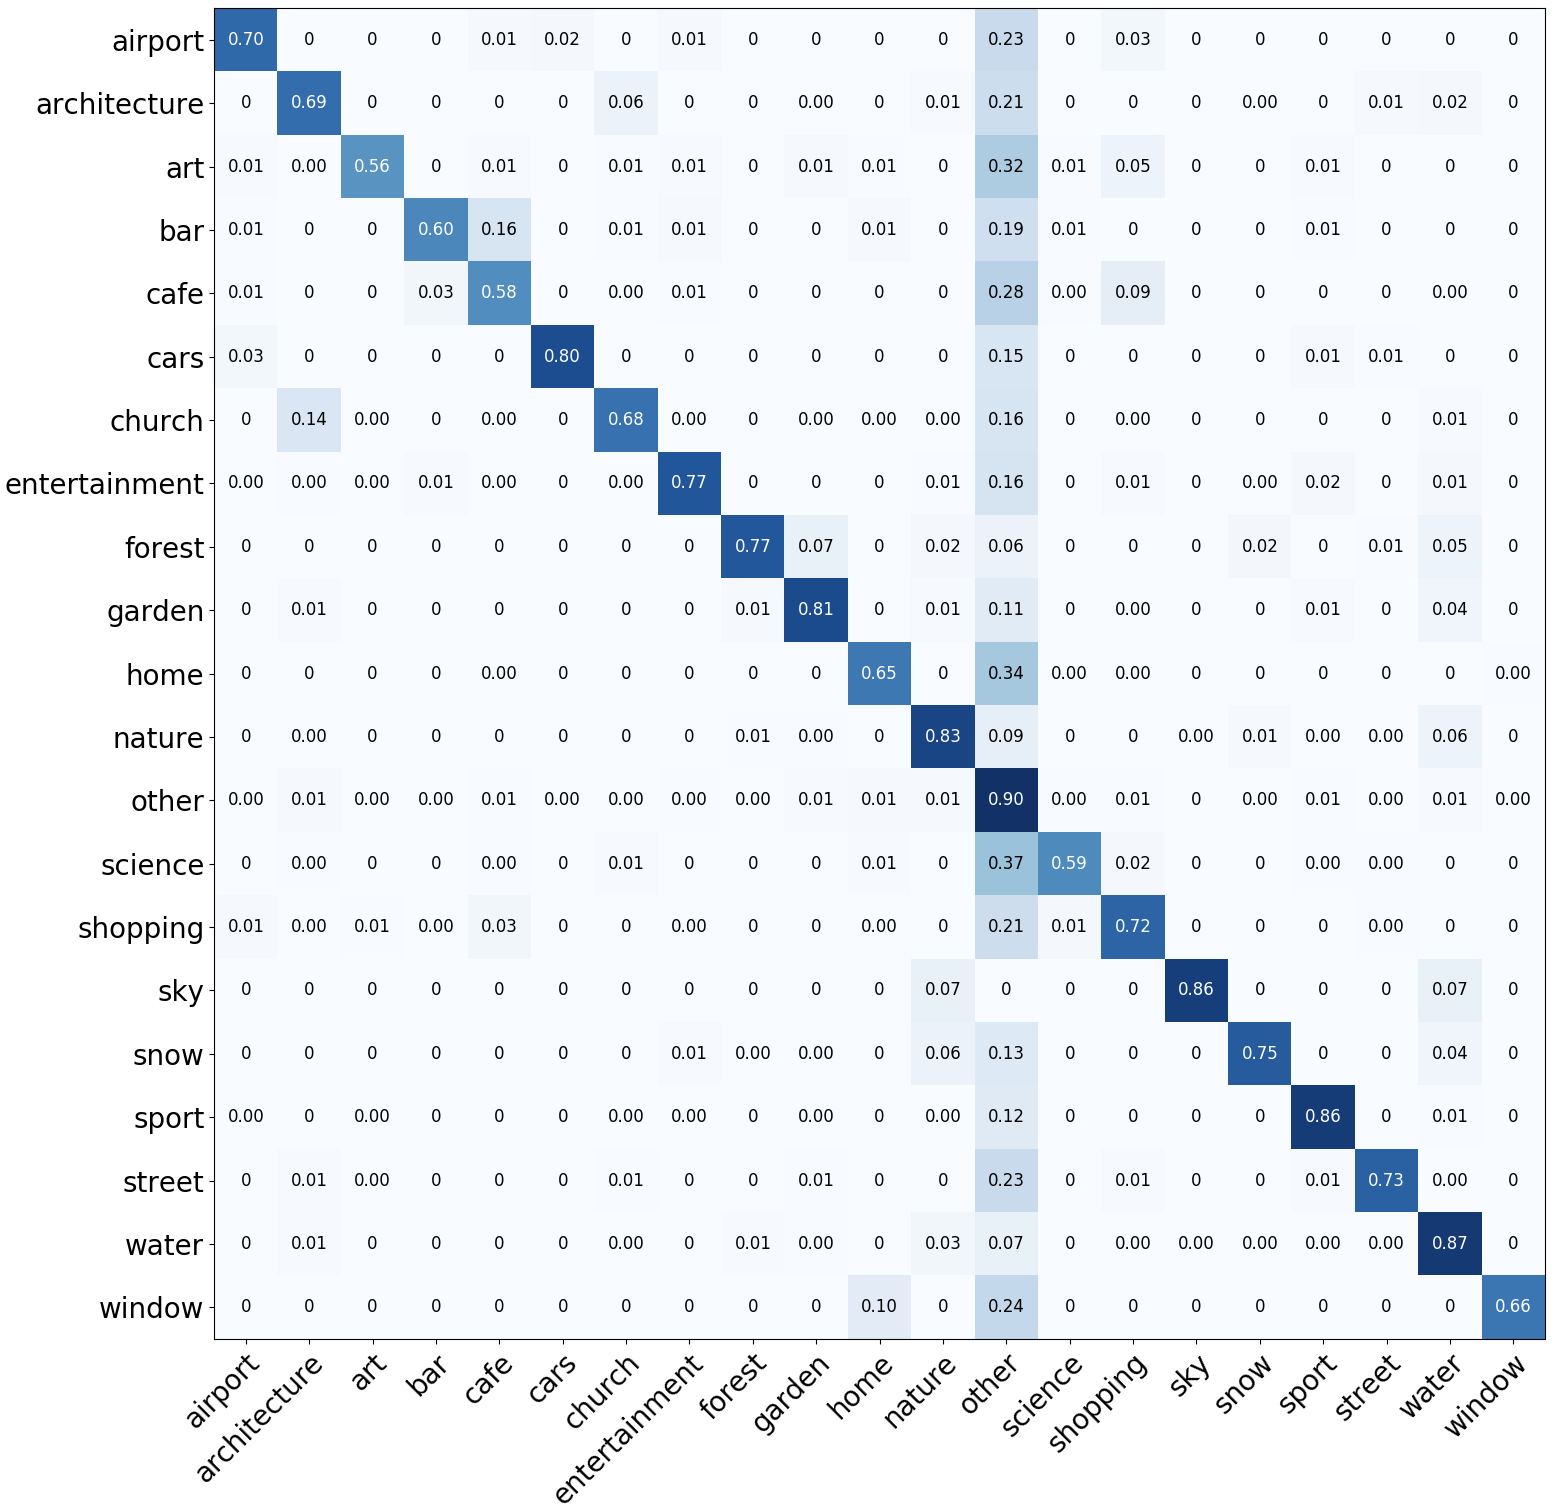
\includegraphics[width=0.98\linewidth]{conf_mat}
   	\end{center}
   	\caption{Матрица ошибок (\textit{confusion matrix}). Истинные метки 
   	               классов отложены по горизонтали, предсказанные -- по вертикали.}
   	\label{tikzpicture: conf_mat}
\end{figure}


\indent
\indent
Проанализируем матрицу ошибок.
Во-первых, её главная диагональ ярко выражена, что хорошо.
Во-вторых, предсказания класса \textit{other},
занимающего половину всего датасета, часто оказываются не 
точны (тёмная вертикальная полоса на рисунке \ref{tikzpicture: conf_mat}).
Это ожидаемое явление и оно не представляет большой проблемы, так как
мы просто не предложим пользователю какой-то хэштег, хотя могли бы.
Было бы хуже, если бы мы предлагали хэштег в случаях, где его 
быть не должно (такая ситуация соответствовала бы тёмной горизонтальной 
полосе на изображении матрицы ошибок).
Как говорилось ранее, наша цель -- построить модель, которая
предсказывает точно, но редко.
В-третьих, можно заметить, что путаются похожие классы, 
некоторые представители
которых могут быть отнесены к нескольким классам одновременно.
Например, \textit{church} и \textit{architecture}; \textit{bar} и \textit{cafe};
\textit{nature} и \textit{water}.


\indent
\indent
Наконец, посмотрим, какие теги предсказала модель для конкретных
примеров из тестовой выборки. Корректные предсказания изображены
на рисунке \ref{tikzpicture: correct_predict}, а неправильные -- на
\ref{tikzpicture: err_predict}. Отобраны примеры, для которых сеть сделала
предсказания с наибольшим значением уверенности.
На рисунке \ref{tikzpicture: err_predict} видна
проблема для классов, упомянутых выше: модель ошибается на примерах, 
которые могли бы быть отнесены сразу к нескольким классам.


\begin{figure}
    \begin{center}
   	    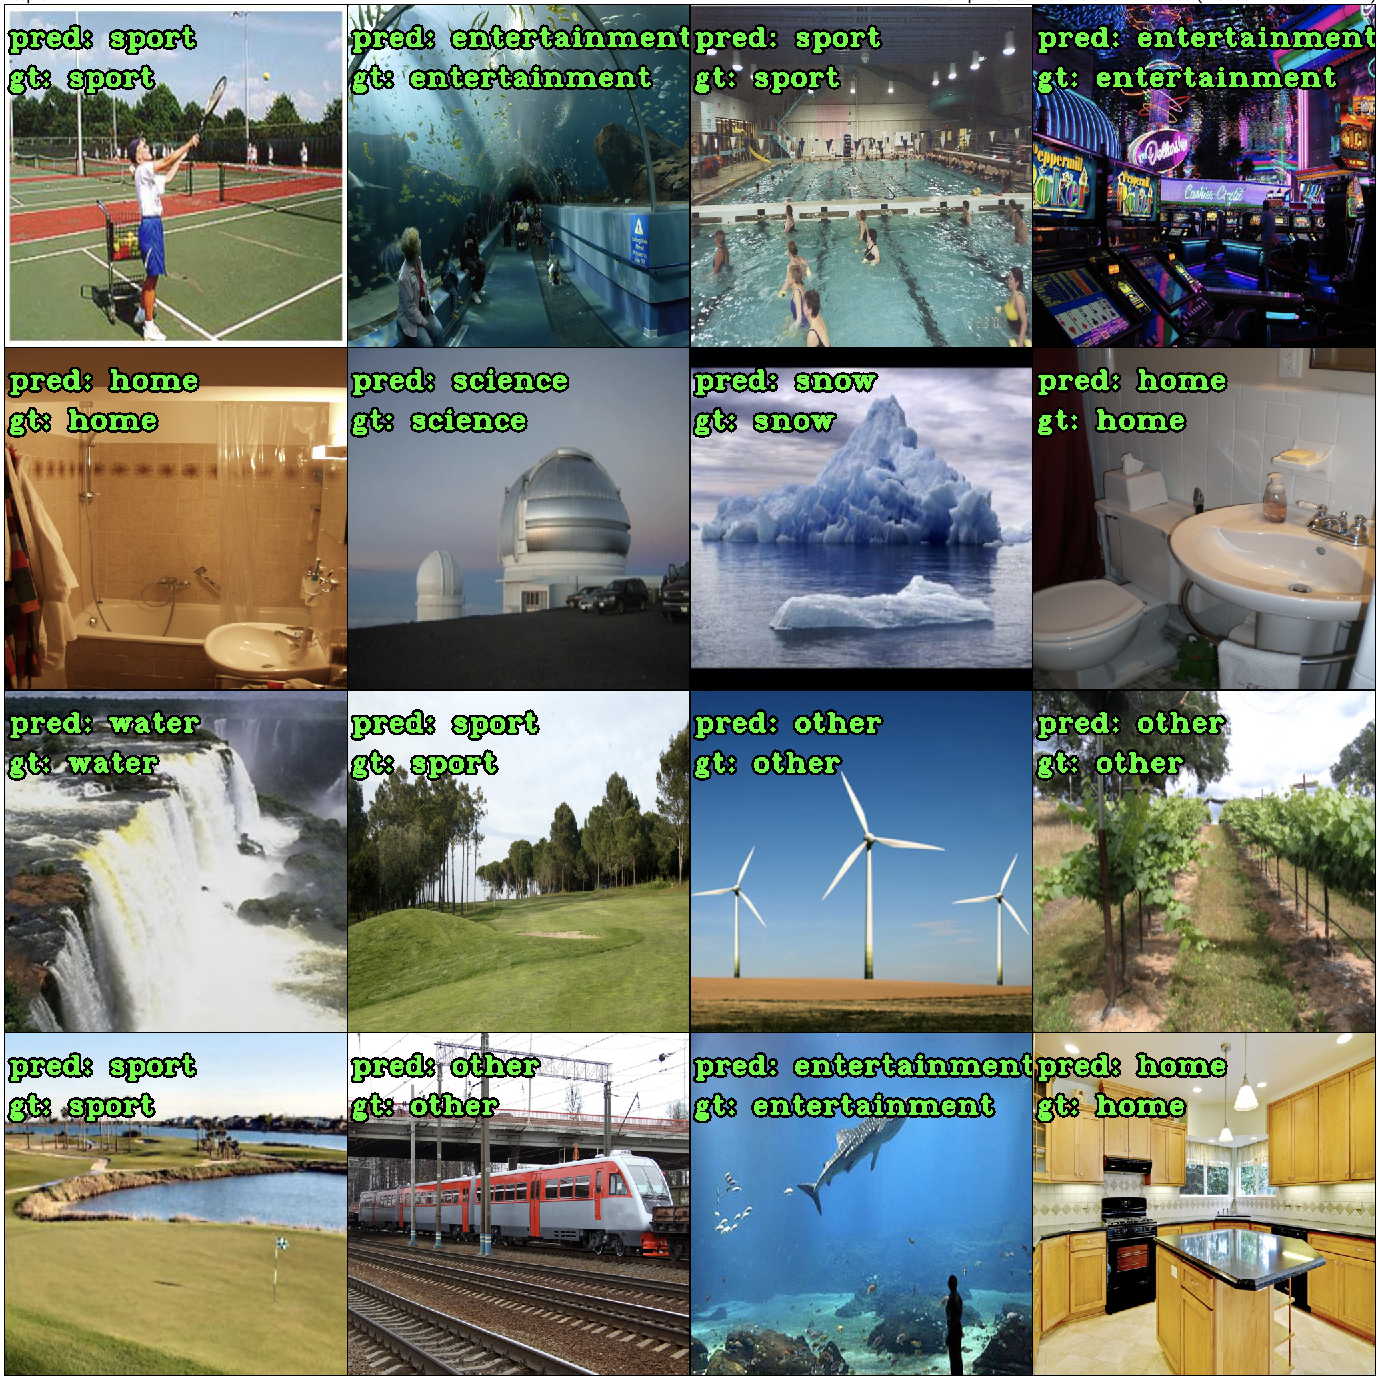
\includegraphics[width=0.9\linewidth]{correct_predict}
   	\end{center}
   	\caption{Примеры, для которых предсказанные
   	 \textit{(predicted)} и истинные \textit{(ground truth)} классы совпадают.}
   	\label{tikzpicture: correct_predict}
\end{figure}


\begin{figure}
    \begin{center}
   	    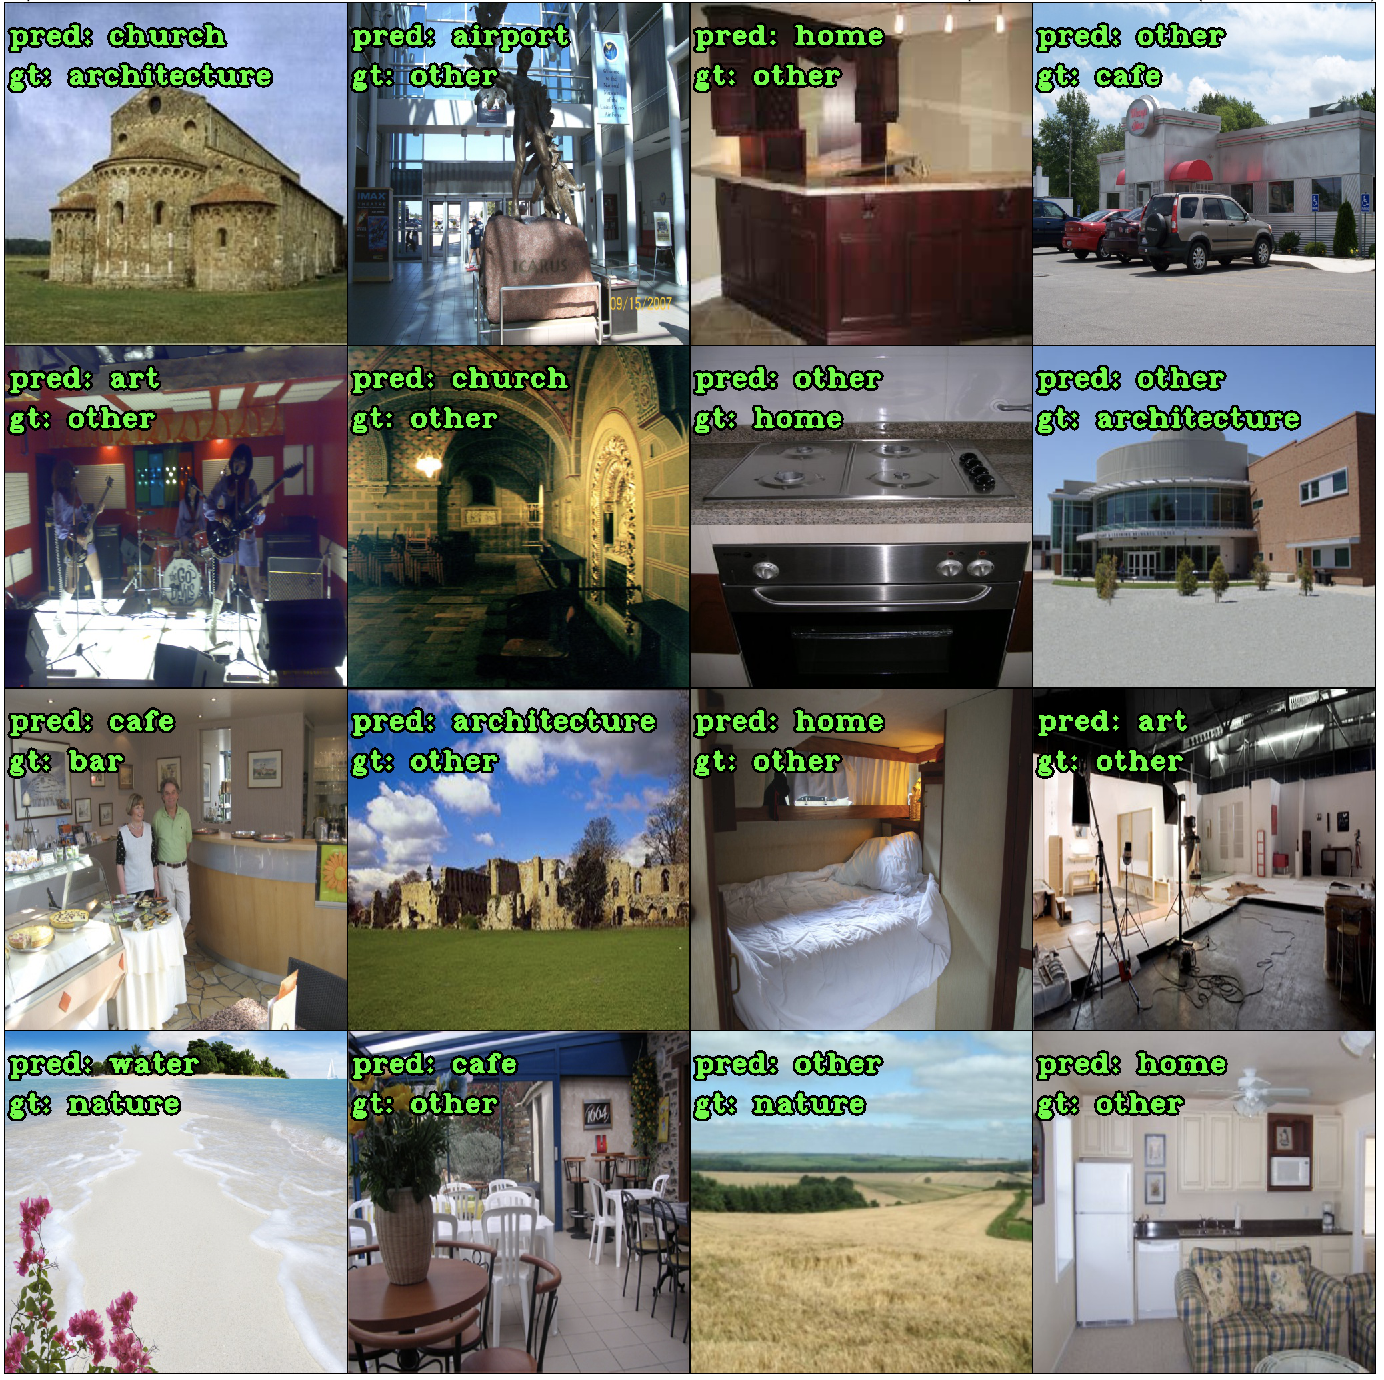
\includegraphics[width=0.9\linewidth]{err_predict}
   	\end{center}
   	\caption{Примеры, для которых предсказанные
   	 \textit{(predicted)} и истинные \textit{(ground truth)} классы не совпадают.}
   	\label{tikzpicture: err_predict}
\end{figure}



\newpage
\section{Валидация результатов}


\newpage
\section*{Выводы}
\addcontentsline{toc}{section}{\tocsecindent{Выводы}}


\newpage
\addcontentsline{toc}{section}{\tocsecindent{Список литературы}}
\begin{thebibliography}{99}

	\bigskip
	
	\bibitem{imagenet}
	Olga Russakovsky, Jia Deng, Hao Su, Jonathan Krause, Sanjeev Satheesh, 
	Sean Ma, Zhiheng Huang, Andrej Karpathy, Aditya Khosla, Michael Bernstein, 
	Alexander C. Berg and Li Fei-Fei. [2015] \textit{ImageNet Large Scale
	 Visual Recognition Challenge}. IJCV.
	 % http://ai.stanford.edu/~olga/bibtex/ILSVRC15.bib
	 
	 
	
\end{thebibliography}


\end{document} 
